\chapter{Ньютоновская космология и уравнение Фридмана}

В прошлый раз мы говорили о метрике пространства. Следующий вопрос — динамика: как масштабный фактор меняется со временем? Сначала немного геометрии, а затем ньютоновская космология. Уравнение Фридмана мы пока не будем выводить из общей теории относительности. Мы выведем его из уравнений Ньютона.

\section{Однородность, изотропия и зависящая от времени метрика}

Однородность и изотропия — основные предположения. Если Вселенная однородна и изотропна и при этом меняется со временем, то закон Хаббла верен всегда. В любой фиксированный момент времени скорость удаления пропорциональна расстоянию,
\begin{equation}
v = H(t)\,d.
\end{equation}
Эта пропорциональность линейна. Постоянство относится не ко времени, а к пространству: в любой данный момент один и тот же коэффициент пропорциональности действует всюду.

\begin{classroomqa}
\audiencequestion{Это означает линейную пропорциональность?}\lecturetimestamp{00:02:06}
\lecturerresponse{Да. При фиксированном времени скорость удаления линейно пропорциональна расстоянию. Коэффициент пропорциональности — это постоянная Хаббла. Вообще говоря, она зависит от времени, но не меняется от точки к точке в пространстве.}
\end{classroomqa}

Именно поэтому выражение ``постоянная Хаббла'' опасно. Она постоянна по отношению к положению в пространстве. По отношению ко времени она не постоянна.

Далее возникает естественный вопрос. Если пространство расширяется, почему тогда не расширяются и метровые стержни? Ответ состоит в том, что метровые стержни удерживаются силами, несравнимо более сильными, чем что-либо, связанное с космологическим расширением на атомных масштабах. Связанные объекты остаются связанными. Расширяется расстояние между достаточно несвязанными объектами, например между галактиками, достаточно далекими друг от друга, чтобы они не связывали друг друга достаточно сильно.

\begin{classroomqa}
\audiencequestion{Нет ли тут проблемы из-за того, что измерительные стержни тоже расширяются?}\lecturetimestamp{00:04:00}
\lecturerresponse{Нет. Измерительные стержни не расширяются. Расширяются координаты. Силы, которые удерживают метровые стержни вместе, гораздо сильнее эффектов, обусловленных расширением, поэтому обычные связанные объекты не расширяются вместе с фоном. Галактики, находящиеся достаточно далеко друг от друга, расходятся, а метровые стержни — нет.}
\end{classroomqa}

Можно даже вообразить крошечный дополнительный отталкивающий эффект между атомами. Но и это не разорвало бы стержень. Это лишь немного сдвинуло бы равновесное расстояние — так же, как небольшое дополнительное натяжение меняет положение равновесия жесткой пружины.

\begin{classroomqa}
\audiencequestion{Но ведь нельзя моделировать это как силу между точками, верно? Потому что иначе это было бы ускорение.}\lecturetimestamp{00:05:29}
\lecturerresponse{Можно вообразить небольшую дополнительную силу между атомами, но если она мала по сравнению с силами связи, то она лишь слегка смещает положение равновесия. Само по себе расширение не порождает обычного закона силы. Некоторые виды расширения можно моделировать через силу, а именно ускоренное расширение, но это мы обсудим позже.}
\end{classroomqa}

Поэтому полезно пользоваться координатами, встроенными в расширяющееся распределение вещества. Галактики, не имеющие дополнительного пекулярного движения, сохраняют одни и те же координатные значения. Со временем меняется соотношение между координатным расстоянием и физическим расстоянием, измеряемым в метрах. Это соотношение задается масштабным фактором \(a(t)\).

Для плоского пространства пространственная метрика может быть записана в виде
\begin{equation}
ds^2 = a(t)^2\left(dx^2+dy^2+dz^2\right).
\end{equation}
Здесь \(a\) — это фактическое расстояние, измеряемое в метрах, между соседними точками, координатное расстояние между которыми равно единице. Если Вселенная расширяется, \(a\) становится зависящим от времени.

Чтобы перейти к пространству-времени, начнем со специальнорелятивистской формы
\begin{equation}
d\tau^2 = dt^2 - ds^2,
\end{equation}
и подставим пространственную метрику. Получаем
\begin{equation}
d\tau^2 = dt^2 - a(t)^2\left(dx^2+dy^2+dz^2\right).
\end{equation}
Коэффициенты не зависят от положения в пространстве. Они зависят только от времени. В языке метрики это и есть утверждение однородности. Диагональная метрика имеет вид
\begin{equation}
g_{\mu\nu}=\mathrm{diag}\!\left(1,-a(t)^2,-a(t)^2,-a(t)^2\right).
\end{equation}
\editorialnote{Полная диагональная матрица, записанная здесь, соответствует устному описанию метрического тензора около 00:14:33. На кадре с доской элемент линии виден ясно, но полностью разборчивая матрица не читается.}

Внедиагональных членов нет. Нет ни \(dx\,dy\), ни \(dx\,dt\), ни других смешанных членов. Метрика почти так же проста, как метрика плоского пространства-времени. Особенность состоит в том, что сама связь между пространственными расстояниями и временем зависит от времени.

\begin{figure}
\centering
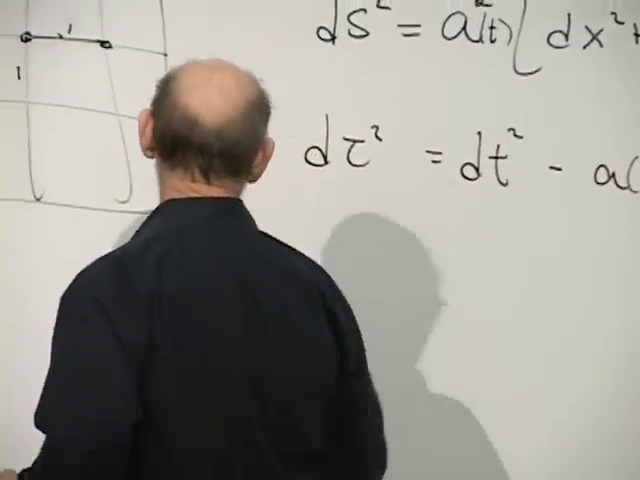
\includegraphics[width=0.62\textwidth]{lecture_02_figure_02.png}
\caption{Эскиз сопутствующей координатной сетки и пространственно-временной интервал с зависящим от времени масштабным фактором.}
\end{figure}

Рисунок передает суть. Алиса и Боб остаются на расстоянии одной единицы друг от друга в сопутствующих координатах, но эта одна координатная единица по мере течения времени соответствует все большему числу метров. Если бы \(a(t)\) в какой-то момент в прошлом был равен нулю, то всякое физическое расстояние было бы равно нулю. Все было бы сплющено одно на другое. Вот почему \(a\to 0\) соответствует бесконечной плотности. Если \(a\) растет, Вселенная становится все более разреженной.

Эта форма метрики справедлива не в любой системе отсчета. Это форма в системе отсчета, движущейся вместе с галактиками.

\begin{classroomqa}
\audiencequestion{В том уравнении маленькое \(t\) в \(a(t)\) — чье это \(t\)?}\lecturetimestamp{00:19:19}
\lecturerresponse{Это время, измеряемое часами, движущимися вместе с галактиками. Представьте себе одинаковые часы, изготовленные на одной и той же космической часовой фабрике и несомые галактиками. В этой системе отсчета временная переменная — в точности то, что измеряют эти часы. Вдоль мировой линии галактики собственное время совпадает с этим координатным временем.}
\end{classroomqa}

Действительно, вдоль мировой линии сопутствующей галактики,
\begin{equation}
dx=dy=dz=0,
\end{equation}
так что
\begin{equation}
d\tau^2 = dt^2,
\end{equation}
и, следовательно,
\begin{equation}
dt=d\tau.
\end{equation}

\begin{classroomqa}
\audiencequestion{Существуют ли преобразования, оставляющие эту форму метрики инвариантной?}\lecturetimestamp{00:23:08}
\lecturerresponse{Повороты — да, потому что \(dx^2+dy^2+dz^2\) инвариантно относительно поворотов. Но бусты Лоренца эту форму не сохраняют. Само вещество выделяет систему отсчета, движущуюся вместе с галактиками, и в какой-нибудь другой системе мир не выглядел бы изотропным.}
\end{classroomqa}

\section{Тело, брошенное в гравитационном поле}

Прежде чем применять механику Ньютона ко всей Вселенной, полезно вернуться к более простой задаче: тяжелая масса \(M\), гораздо меньшая масса \(m\) и начальный толчок наружу. После этого толчка малая масса просто движется в гравитационном поле и ведет себя так, как велят уравнения Ньютона.

Для космологического обсуждения важно не полное решение задачи об орбите. Важно сохранение энергии. Кинетическая энергия равна
\begin{equation}
\frac{1}{2}mv^2.
\end{equation}

\begin{figure}
\centering
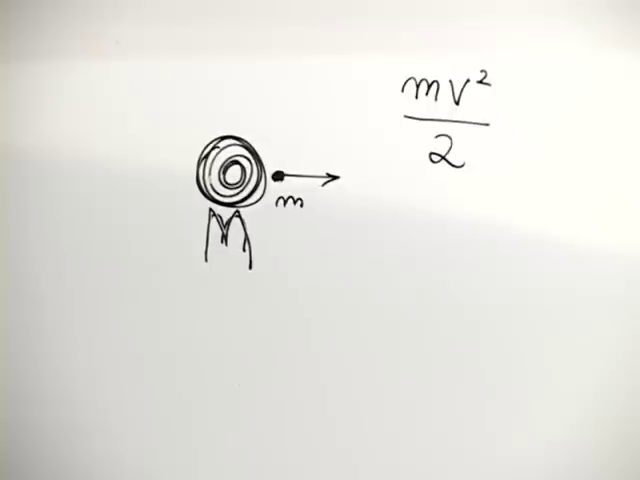
\includegraphics[width=0.42\textwidth]{lecture_02_figure_03.png}
\caption{Удаляющаяся пробная масса и член кинетической энергии \(\frac{1}{2}mv^2\).}
\end{figure}

Гравитационная потенциальная энергия содержит произведение масс, постоянную Ньютона и расстояние в первой степени в знаменателе. В записи на доске множители идут в порядке \(mMG/D\), поэтому лучше сохранить здесь этот порядок:
\begin{equation}
-\frac{mMG}{D}.
\end{equation}
Тогда полная энергия равна
\begin{equation}
\frac{1}{2}mv^2-\frac{mMG}{D}.
\end{equation}
Закон сохранения энергии утверждает лишь, что для рассматриваемой конкретной частицы эта величина не меняется со временем. У разных частиц энергии могут быть разными.

\begin{figure}
\centering
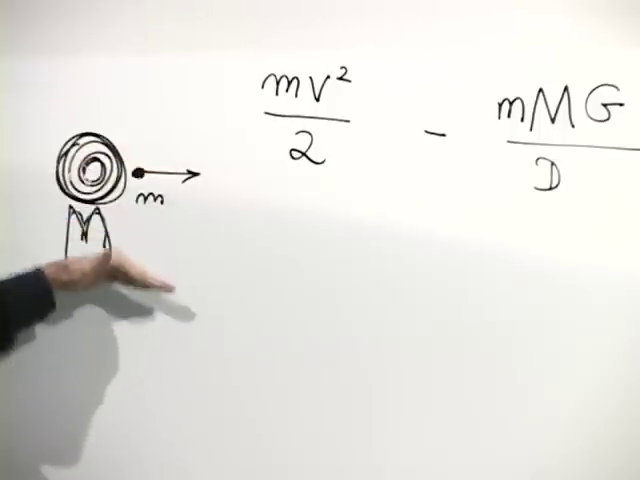
\includegraphics[width=0.62\textwidth]{lecture_02_figure_04.png}
\caption{Полная ньютоновская энергия для радиально движущейся пробной массы: кинетический член минус член гравитационной потенциальной энергии.}
\end{figure}

Отрицательный знак важен. Гравитационная потенциальная энергия отрицательна, потому что гравитация притягивает. Приближение частицы создает больше отрицательной потенциальной энергии. Перемещение ее дальше делает потенциальную энергию менее отрицательной.

\begin{classroomqa}
\audiencequestion{Потенциальная энергия растет с расстоянием, а не убывает?}\lecturetimestamp{00:34:13}
\lecturerresponse{Да. Отбросьте константы и посмотрите на графики \(1/D\) и \(-1/D\). Сила направлена в сторону убывания потенциальной энергии. Поэтому притягивающей силе соответствует перевернутая кривая, \(-1/D\), так что потенциальная энергия возрастает с расстоянием и становится более отрицательной, когда частица движется внутрь.}
\end{classroomqa}

\begin{figure}
\centering
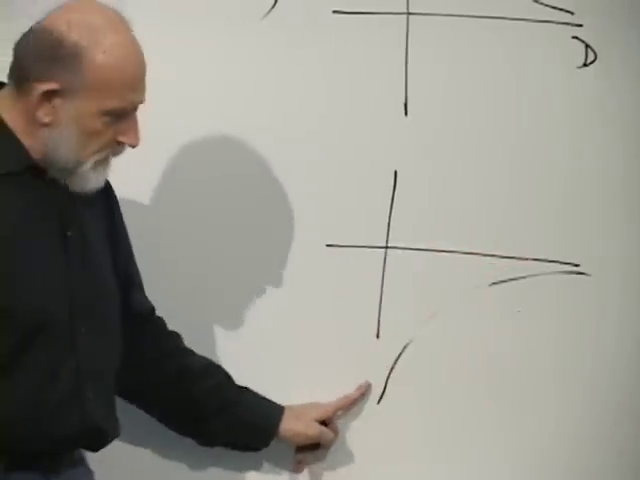
\includegraphics[width=0.46\textwidth]{lecture_02_figure_05.png}
\caption{Качественное сравнение \(1/D\) и \(-1/D\) для знака гравитационной потенциальной энергии.}
\end{figure}

\section{Скорость убегания}

Теперь классифицируем возможности. Энергия может быть положительной, отрицательной или нулевой. Это единственные три случая.

\begin{itemize}
\item Если энергия отрицательна, частица связана. Бросьте ее вверх со слишком малой скоростью, и она поднимется, замедлится, развернется и упадет обратно.
\item Если энергия положительна, частица убегает. Сначала гравитация замедляет ее, но недостаточно, чтобы остановить, и в конце концов она удаляется с ненулевой асимптотической скоростью наружу.
\item Если энергия в точности равна нулю, частица имеет скорость убегания. Это пограничный случай между тем, чтобы убежать, и тем, чтобы не убежать.
\end{itemize}

При достаточно малой начальной скорости с самого начала доминирует потенциальный член, и энергия отрицательна.

\begin{figure}
\centering
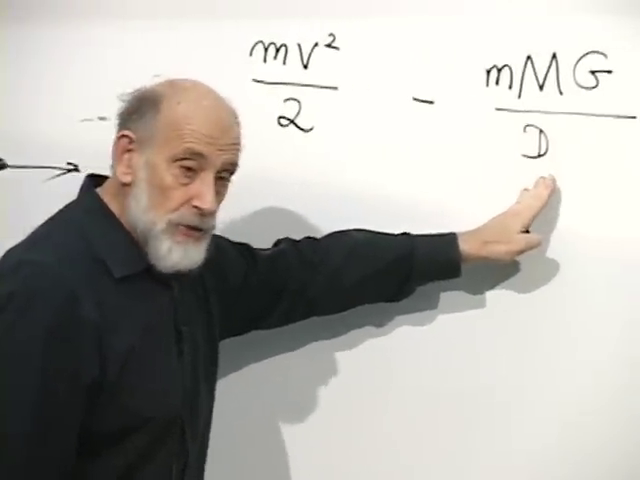
\includegraphics[width=0.62\textwidth]{lecture_02_figure_06.png}
\caption{При малой скорости наружу отрицательный потенциальный член доминирует в полной энергии.}
\end{figure}

В случае нулевой энергии расстояние продолжает увеличиваться, но скорость продолжает уменьшаться. Частица не может остановиться ни в какой конечный момент времени. Если бы это произошло, она упала бы обратно. Поэтому расстояние неограниченно, а скорость стремится к нулю.

Именно эта прямая аналогия важна для космологии. Вселенная может вести себя точно так же. Если начальный направленный наружу хаббловский поток достаточно велик, всё удаляется от всего остального. Если он слишком мал, побеждает гравитация и происходит гигантское сжатие. Есть и предельный случай, в точности аналогичный скорости убегания.

\section{Теорема Ньютона}

Космологическое сведение работает благодаря теореме Ньютона для закона обратных квадратов.

Если вещество распределено сферически симметрично относительно некоторого центра, то гравитационная сила, действующая на частицу вне этого распределения, в точности такая же, как если бы вся масса была сосредоточена в центре. Но теорема сильнее этого. Если частица находится внутри распределения, то вклад дает только масса на меньшем радиусе. Масса на большем радиусе не дает результирующей силы.

Самая ясная версия теоремы — тонкая оболочка. Идеальная сферическая оболочка не действует гравитационно на частицу нигде внутри нее, даже вдали от центра. На первый взгляд это удивительно, но для закона \(1/r^2\) это верно.

\begin{classroomqa}
\audiencequestion{В приведенном вами примере не должно ли нас немного удивлять то, что, когда частица пересекает границу, сила кажется разрывной?}\lecturetimestamp{00:48:19}
\lecturerresponse{Да. Для идеальной бесконечно тонкой оболочки это удивительно, и это свойственно именно закону силы \(1/r^2\). Реальная оболочка имеет толщину, поэтому изменение сглаживается, но резкое утверждение для идеальной оболочки и есть в точности замечательное свойство теоремы Ньютона.}
\end{classroomqa}

Тогда наглядный рисунок делает теорему правдоподобной. Замените точечную массу точечным источником воды. В трех измерениях поток наружу убывает как \(1/r^2\). Расположите такие источники непрерывно по всей сферической оболочке. Вне оболочки поток выглядит в точности так, как если бы всё было сосредоточено в центре. Внутри оболочки не может быть никакого результирующего потока, потому что в центре нет источника. Именно эта структура лежит и в основе гравитационной теоремы.

Смысл здесь не в том, чтобы заново выводить теорему. Смысл в том, чтобы ею пользоваться.

\section{Однородная Вселенная как задача об одном теле}

Теперь вернемся к космологии. Возьмите небольшой участок мира, заполненный однородным газом галактик. При желании можно считать себя находящимся в центре. Это лишь удобство. Любой может считать себя находящимся в центре, и должно получиться то же самое уравнение.

Выберите галактику на оси \(x\) с сопутствующей координатой \(x\). Поскольку Вселенная изотропна, выбор оси несуществен. Проведите сферу с центром в \(x=0\), проходящую через эту галактику. По теореме Ньютона сила, действующая на галактику, в точности такая же, как если бы вся масса внутри этой сферы была сосредоточена в центре, тогда как всё снаружи не давало никакого вклада.

Сфера расширяется вместе с галактиками. Она всегда содержит одни и те же галактики и, следовательно, ту же суммарную массу, хотя ее физический радиус меняется со временем.

Поэтому движение этой галактики подчиняется в точности такому же уравнению энергии, как и у снаряда:
\begin{equation}
\frac{1}{2}mv^2-\frac{mMG}{D}=\text{constant}.
\end{equation}
Здесь \(M\) теперь означает массу внутри расширяющейся сферы, а не центральную массу во вводном примере. Алгебра затем упрощается, если умножить на \(2\) и разделить на \(m\). Поскольку константа, деленная на \(m\), все равно остается просто константой, можно написать
\begin{equation}
v^2-\frac{2MG}{D}=\text{constant}.
\end{equation}
И снова ``константа'' означает константу по времени для данной конкретной галактики.

Теперь свяжем это с масштабным фактором. Физическое расстояние до галактики равно
\begin{equation}
D=ax,
\end{equation}
поскольку \(x\) — фиксированная сопутствующая координата. Скорость галактики равна
\begin{equation}
v=\dot D=\dot a\,x.
\end{equation}

Масса внутри сферы равна плотности, умноженной на объем. Если \(\rho\) — массовая плотность, то
\begin{equation}
M=\frac{4\pi}{3}\rho D^3=\frac{4\pi}{3}\rho a^3x^3.
\end{equation}
Подстановка в уравнение энергии дает
\begin{equation}
\dot a^2x^2-\frac{2G}{ax}\left(\frac{4\pi}{3}\rho a^3x^3\right)=\text{constant},
\end{equation}
или
\begin{equation}
\dot a^2x^2-\frac{8\pi G}{3}\rho a^2x^2=\text{constant}.
\end{equation}

Оба члена в левой части пропорциональны \(x^2\). Все остальное здесь одинаково повсюду. Следовательно, правая часть тоже должна быть пропорциональна \(x^2\). Это не противоречит тому, что ее называют константой. Это означает константу по времени для каждого фиксированного \(x\), но от одной галактики к другой она все же может масштабироваться как \(x^2\). В этом есть смысл. Более далекие галактики движутся быстрее.

Поэтому разделим на общий множитель \(x^2\). Оставшаяся константа теперь не зависит ни от времени, ни от пространства. Исторически стандартно обозначим ее как \(-k\):
\begin{equation}
\dot a^2-\frac{8\pi G}{3}\rho a^2=-k.
\end{equation}
После деления на \(a^2\)
\begin{equation}
\left(\frac{\dot a}{a}\right)^2=\frac{8\pi G}{3}\rho-\frac{k}{a^2}.
\end{equation}

Это знаменитое уравнение Фридмана—Робертсона—Уокера, хотя в лекции также замечается, что на самом деле это уравнение Фридмана. Соглашение о знаке историческое. То, что пишут \(-k\), не означает, что \(k\) должно быть положительным. \(k\) может быть положительным, отрицательным или нулем. В единицах, где скорость света положена равной \(1\), \(k\) безразмерно.

\section{Плотность и уравнение для случая доминирования вещества}

Следующий вопрос возникает сразу: что такое \(\rho\)? Это не константа. По мере расширения Вселенной плотность уменьшается.

Чтобы выразить эту зависимость, возьмите единичный куб в координатном пространстве: по одной единице по \(x\), \(y\) и \(z\). Внутри этого куба во все времена остаются одни и те же галактики, потому что куб расширяется вместе с координатной сеткой. Поэтому масса внутри этого координатного куба фиксирована.

\editorialnote{В лекции символ \(M\) используется повторно на нескольких этапах. Здесь \(M_{\Box}\) используется только для того, чтобы отличать массу в единичном координатном кубе от ранее встречавшихся центральной массы и массы, заключенной внутри сферы.}

Физическая длина ребра куба равна \(a\), так что его физический объем равен \(a^3\). Следовательно,
\begin{equation}
\rho=\frac{M_{\Box}}{a^3}.
\end{equation}
Это случай доминирования вещества: в правой части фигурирует только плотность обычного нерелятивистского вещества.

\begin{classroomqa}
\audiencequestion{Согласно этому уравнению, постоянная Хаббла является функцией \(\rho\). Следовательно, это не константа.}\lecturetimestamp{01:19:21}
\lecturerresponse{Именно. Постоянная Хаббла не является константой. Она зависит от плотности, а плотность меняется со временем. В лекции даже шутят, что итоговый экзамен мог бы состоять из одного вопроса: является ли постоянная Хаббла константой?}
\end{classroomqa}

Подстановка \(\rho=M_{\Box}/a^3\) в уравнение Фридмана дает
\begin{equation}
\left(\frac{\dot a}{a}\right)^2=\frac{8\pi G M_{\Box}}{3a^3}-\frac{k}{a^2}.
\end{equation}

На этом этапе уже ясно, какие величины выбираются произвольно. Нужно задать массу в единичном координатном кубе и значение \(k\). Трем возможным знакам \(k\) соответствуют три энергетических случая в задаче о снаряде.

\begin{itemize}
\item При \(-k>0\) энергия эффективно выше уровня, соответствующего скорости убегания, и Вселенная расширяется вечно.
\item При \(-k<0\) гравитация в конце концов побеждает, и Вселенная снова коллапсирует.
\item При \(k=0\) имеет место точный аналог скорости убегания.
\end{itemize}

\begin{classroomqa}
\audiencequestion{Если \(k=0\), то скорость между двумя галактиками стремится к нулю?}\lecturetimestamp{01:21:12}
\lecturerresponse{Да. В критическом случае скорость стремится к нулю, но расстояние все равно неограниченно. Галактики продолжают расходиться, только все медленнее и медленнее. Если бы они действительно остановились в какой-либо конечный момент времени, они упали бы обратно.}
\end{classroomqa}

\section{Критический случай \(k=0\)}

Теперь выберем простейший случай, \(k=0\). Это в точности случай скорости убегания, и он проще лишь потому, что проще математика. Уравнение принимает вид
\begin{equation}
\left(\frac{\dot a}{a}\right)^2=\frac{8\pi G M_{\Box}}{3a^3}.
\end{equation}

Правая часть всегда положительна и никогда не обращается в нуль. Следовательно, \(\dot a/a\) не может пройти через нуль. В этом случае Вселенная не может развернуться. Она либо всегда расширяется, либо всегда сжимается. Возьмем расширяющуюся ветвь.

Теперь предположим степенной закон,
\begin{equation}
a(t)=ct^p.
\end{equation}
Тогда
\begin{equation}
\dot a = cp\,t^{p-1},
\end{equation}
следовательно,
\begin{equation}
\frac{\dot a}{a}=\frac{p}{t}.
\end{equation}
Подстановка в дифференциальное уравнение дает
\begin{equation}
\frac{p^2}{t^2}=\frac{8\pi G M_{\Box}}{3c^3t^{3p}}.
\end{equation}
Чтобы степени \(t\) совпали, должно выполняться
\begin{equation}
3p=2.
\end{equation}
Значит,
\begin{equation}
p=\frac{2}{3}.
\end{equation}
Тогда для констант должно выполняться
\begin{equation}
\frac{4}{9}=\frac{8\pi G M_{\Box}}{3c^3},
\end{equation}
откуда
\begin{equation}
c^3=6\pi G M_{\Box}.
\end{equation}
Следовательно,
\begin{equation}
a(t)=\left(6\pi G M_{\Box}\right)^{1/3}t^{2/3}.
\end{equation}

При этом еще возможен аддитивный сдвиг времени. Он поглощается заменой \(t\) на \(t-t_0\). Как только выбирают начало отсчета времени так, что \(a=0\) при \(t=0\), эта оставшаяся константа исчезает.

Итак, Вселенная расширяется как время в степени две трети,
\begin{equation}
a(t)\propto t^{2/3}.
\end{equation}
Она не расширяется линейно со временем. Линейный рост был бы аналогом движения без ускорения. Здесь расширение замедляется.

Если продолжить формулу назад до \(t=0\), масштабный фактор стремится к нулю, а плотность неограниченно возрастает. Говорить \(a=0\) — это уже крайность. Мы не знаем, что происходит с веществом, когда оно становится слишком плотным. Реальный смысл в том, что на некоторой ранней стадии всё было настолько тесно упаковано, что атомы, ядра и кварки были тесно упакованы в чрезвычайно плотном состоянии.

\section{Постоянная Хаббла и возраст Вселенной}

В критической модели,
\begin{equation}
H(t)=\frac{\dot a}{a}=\frac{2}{3t}.
\end{equation}
Итак, постоянная Хаббла приблизительно равна величине, обратной возрасту Вселенной,
\begin{equation}
t=\frac{2}{3H}.
\end{equation}
Это один из главных результатов вычисления. Измерив сегодня постоянную Хаббла, мы получаем оценку возраста Вселенной, по крайней мере вплоть до того момента, когда ньютоновская модель перестает иметь смысл.

Указанный возраст составляет примерно от \(13\) до \(14\) миллиардов лет. В тексте также сказано, что \(k=0\) очень реалистично с точки зрения наблюдений: при указанной там точности никакого существенного отклонения от \(k=0\) не известно.

\begin{classroomqa}
\audiencequestion{Я просто немного запутался в том, что такое \(M\) и \(a\).}\lecturetimestamp{01:39:16}
\lecturerresponse{Обе величины содержат произвольность, связанную с выбором сетки. Если изменить условно выбранный ящик, изменится количество вещества в нем, и численное значение масштабного фактора тоже изменится. Физический смысл имеет плотность, \(M/a^3\), или, эквивалентно, комбинации вроде \(a/M^{1/3}\), которые не зависят от того, как выбрана сетка. В решении с \(k=0\) неизвестная постоянная, множащая \(t^{2/3}\), сокращается в \(\dot a/a\), так что соотношение для возраста \(t=2/3H\) не зависит от массы вещества в этом ящике.}
\end{classroomqa}

Это сокращение видно непосредственно из решения. Если
\begin{equation}
a(t)=Ct^{2/3},
\end{equation}
то
\begin{equation}
\dot a=\frac{2}{3}Ct^{-1/3},
\end{equation}
и, следовательно,
\begin{equation}
\frac{\dot a}{a}=\frac{2}{3t}.
\end{equation}
Постоянная \(C\) полностью сокращается.

\section{Почему ньютоновский вывод работает}

Ближе к концу возникает вопрос: почему ньютоновский вывод должен так хорошо согласовываться с релятивистским?

\begin{classroomqa}
\audiencequestion{Похоже, что все это зависит от предположения об открытой Вселенной.}\lecturetimestamp{01:45:44}
\lecturerresponse{На этом этапе вывод ньютоновский, а ньютоновская физика означает плоское пространство. Интерпретация \(k\) в терминах геометрии пространства отложена до следующей лекции. Там \(k=0\) будет соответствовать плоскому пространству, тогда как другие знаки будут связаны с искривленной пространственной геометрией.}
\end{classroomqa}

\begin{classroomqa}
\audiencequestion{Зависела ли когда-то очень давно длина метровых стержней от \(a\)?}\lecturetimestamp{01:47:53}
\lecturerresponse{Если уйти достаточно далеко в прошлое, вещество было бы настолько скучено, что отдельных метровых стержней на самом деле не существовало бы. А до того они были бы сжаты вместе. Лекция также напоминает, что теория относительности и так не допускает по-настоящему жестких тел: если бы тело было совершенно жестким, толчок с одной стороны мгновенно передавал бы сигнал на другую сторону, быстрее света.}
\end{classroomqa}

\begin{classroomqa}
\audiencequestion{Почему, как вы думаете, имеется такое совпадение между уравнениями — ньютоновским и релятивистским?}\lecturetimestamp{01:49:03}
\lecturerresponse{Потому что ньютоновское рассмотрение применяется лишь к достаточно малой области. Пока эта область мала по сравнению с радиусом кривизны всей Вселенной и пока локальные скорости Хаббла в ней значительно меньше скорости света, ньютоновская механика является хорошим приближением. В лекции это сравнивается с изучением роста травы на Земле: локальный процесс можно понять, не привлекая кривизну всей Земли.}
\end{classroomqa}

Это и есть логика локальной области. Ньютоновская механика предполагает, во-первых, что кривизна пространства не важна для рассматриваемого вопроса, и, во-вторых, что локально ничто не движется со скоростью, близкой к скорости света. В космологии это означает выбрать область, достаточно большую, чтобы быть однородной, но все же достаточно малую, чтобы эффектами кривизны можно было пренебречь и скорости Хаббла оставались нерелятивистскими.

Имея это в виду, ньютоновский расчет — не случайность. Это локальное приближение к уравнению, которое можно записать и в релятивистской форме. Если член кривизны перенести в левую часть, уравнение Фридмана принимает вид
\begin{equation}
\left(\frac{\dot a}{a}\right)^2+\frac{k}{a^2}=\frac{8\pi G}{3}\rho.
\end{equation}
Левая часть геометрична: в нее входят масштабный фактор и, как мы увидим в следующий раз, кривизна пространства. Правая часть — это плотность энергии. Именно такого рода уравнения и следует ожидать от общей теории относительности.

В следующий раз темой будут сама кривизна, уравнения Эйнштейна и связь между этим релятивистским выводом и ньютоновским.